% =====================================================================
%  Data Mining · SGH · SMMD-ADA / SMMD-AAB   —   Block 2 slide deck
%  Template: Frankfurt + seahorse + miniframes (same as course template)
%
%  Compilation:
%    pdflatex block2.tex   (run twice for the section headline)
%
%  Figures: regenerate with   uv run python lecture_2/make_figures.py
%
%  Speaker-notes display modes (uncomment one):
%    \setbeameroption{hide notes}                          % slides only
%    \setbeameroption{show notes}                          % slides + note pages
%    \setbeameroption{show notes on second screen=right}   % presenter mode
%    \setbeameroption{show only notes}                     % notes printout
% =====================================================================
\documentclass[10pt,aspectratio=169]{beamer}

\usepackage[utf8]{inputenc}
\usepackage[T1]{fontenc}
\usepackage{booktabs}
\usepackage{array}
\usepackage{multirow}
\usepackage{amsmath,amssymb}
\usepackage{graphicx}
\usepackage{xcolor}
\usepackage{tikz}
\usetikzlibrary{arrows.meta,positioning,shapes.geometric}

% - Theme -
\usetheme{Frankfurt}
\usecolortheme{seahorse}
\useoutertheme{miniframes}
\setbeamertemplate{navigation symbols}{}
\setbeamertemplate{footline}[frame number]

% - Speaker notes -
\setbeameroption{hide notes}
% \setbeameroption{show notes on second screen=right}

% - Colours for figures -
\definecolor{sghblue}{RGB}{0,51,102}

% - Metadata -
\title[Data Mining]{Data Mining}
\subtitle{Block 2 - Regression, re-framed: from inference to prediction}
\author{Daniel Wlazło}
\institute{SGH Warsaw School of Economics - SMMD-ADA / SMMD-AAB}
\date{13 October 2026}

\begin{document}

% ============================================================
% TITLE SLIDE
% ============================================================
\begin{frame}[plain]
  \begin{center}
    \vspace{1cm}
    {\LARGE\textbf{Data Mining}}\\[0.5cm]
    {\large Block 2 - Regression, re-framed: from inference to prediction}\\[1.5cm]
    {\large Daniel Wlazło} \\[0.2cm]
    {\small SGH Warsaw School of Economics - SMMD-ADA / SMMD-AAB} \\[0.2cm]
    {\small 13 October 2026}
  \end{center}
\end{frame}

% ============================================================
\begin{frame}{Today, hour by hour}
  \begin{enumerate}\small
    \item \textbf{Recap} - what Block 1 left on the table \hfill {\small$\sim$5 min}
    \item \textbf{Why these models} - in the age of LLMs \hfill {\small$\sim$10 min}
    \item \textbf{Tools} - scikit-learn; train / validation / test \hfill {\small$\sim$10 min}
    \item \textbf{From inference to prediction} - overfitting, the split protocol \hfill {\small$\sim$15 min}
    \item \textbf{Linear regression} - as a prediction machine \hfill {\small$\sim$30 min}
    \item \textbf{Logistic regression} - the credit-scoring workhorse \hfill {\small$\sim$35 min}
    \item \textbf{Regularisation} - ridge, lasso, and why scaling matters \hfill {\small$\sim$20 min}
    \item \textbf{Evaluating classifiers, part 1} - beyond accuracy \hfill {\small$\sim$20 min}
    \item \textbf{Lab} - notebook \texttt{02\_regression\_baselines} \hfill {\small$\sim$35 min}
  \end{enumerate}
  \vspace{0.4em}
  \begin{center}\small Breaks roughly every 50 minutes.\end{center}
\end{frame}

% ============================================================
\begin{frame}{Last week in five sentences}
  \begin{enumerate}
    \item Data mining starts from a \textbf{decision}; translating it into a
          learning task is your job.
    \item \textbf{EDA before models}: target balance, distributions,
          bivariate reads - and always plot.
    \item Missingness has a \textbf{mechanism}; the mechanism dictates the
          treatment.
    \item The \texttt{delinq\_missing} \textbf{indicator} we engineered carries
          more default signal than any raw numeric column.
    \item Every feature must pass the \textbf{time-travel test} -
          application-time information only.
  \end{enumerate}
  \vspace{0.5em}
  \begin{center}
    Today the craft graduates to a \alert{real} portfolio - and we watch
    which lessons transfer. (Spoiler: engineered delay counters become the
    new star.)
  \end{center}
\end{frame}

% ============================================================
\begin{frame}{Where we are on the map}
  \small
  \begin{center}
  \begin{tabular}{@{}lp{4.2cm}p{4.4cm}@{}}
    \toprule
    Task & Target & Today's example \\
    \midrule
    \textbf{Regression} & a number & payments from bills (warm-up) \\
    \textbf{Binary classification} & two classes & \alert{probability of default} \\
    \bottomrule
  \end{tabular}
  \end{center}
  \vspace{0.6em}
  \begin{itemize}\small
    \item Both of today's tools are \emph{linear models} - one line of
          mathematics apart.
    \item They are also the \alert{baselines} every fancier model of this
          course must beat to justify itself.
  \end{itemize}
\end{frame}

% ============================================================
\begin{frame}{Meet the real portfolio}
  From today on, the modelling blocks run on \alert{real data}:
  \vspace{0.3em}
  \begin{itemize}\small
    \item \textbf{30{,}000 credit-card clients} of a Taiwanese bank (2005)
          - the classic UCI \emph{Default of Credit Card Clients} study
          (Yeh \& Lien). Target: \texttt{default} next month -
          base rate \alert{22.1\%}.
    \item Columns: credit limit, demographics (sex, age, education,
          marriage), and \alert{six months of behaviour} - repayment
          status, bill amounts, payment amounts.
    \item Loaded via \texttt{finance\_data.load\_taiwan()} - downloaded
          once, cached in the repo, works offline.
    \item One column is \alert{planted and documented}:
          \texttt{collections\_contact}, injected exactly like in Block 1's
          synthetic portfolio. You know the drill - and Block 3 pulls the
          pin.
  \end{itemize}
  \vspace{0.3em}
  \begin{center}\small
    Block 1's synthetic portfolio retires to the missingness lab - real
    data never labels its missingness mechanisms; ours did, by design.
  \end{center}
\end{frame}

% ============================================================
% SECTION: WHY THESE MODELS
% ============================================================
\section{Why}

% ---------------------------------------------------------------
\begin{frame}{Why bother, in the age of LLMs?}
  A fair question: ChatGPT exists - why learn logistic regression?
  \vspace{0.3em}
  \begin{itemize}\small
    \item \textbf{Structured data is not language.} On tabular problems
          (a credit portfolio is one), small dedicated models still
          \alert{match or beat} LLMs - at a millionth of the cost per
          decision.
    \item \textbf{Explainability is a legal requirement.} A declined customer
          is entitled to reasons; ``the LLM said so'' is not one.
          Coefficients and odds ratios are.
    \item \textbf{Regulation.} Credit models live under model-risk
          frameworks: validated, monitored, auditable, reproducible.
          A deterministic model with fixed coefficients can be audited;
          a prompt cannot.
    \item \textbf{Insight.} The point is often the \emph{drivers}, not the
          prediction: which behaviours signal risk? A coefficient answers;
          a chat completion gestures.
    \item \textbf{Latency, cost, stability.} Millions of scoring calls per
          day, identical answer for identical input, fractions of a cent.
  \end{itemize}
\end{frame}

% ---------------------------------------------------------------
\begin{frame}{Where LLMs \emph{do} fit in this course's world}
  \begin{itemize}
    \item \textbf{As your assistant}: writing pandas code, explaining
          errors, drafting documentation - use them for the lab, and
          \alert{verify what they produce} (Block 1: reading errors).
    \item \textbf{As feature factories}: turning complaint texts into
          categories or embeddings that feed a \emph{classical} model -
          exactly Block 5's text-mining pipeline, modern edition.
    \item \textbf{Not as the decision engine} for regulated, high-volume,
          structured decisions - for the reasons on the previous slide.
  \end{itemize}
  \vspace{0.6em}
  \begin{block}{The division of labour}
    LLMs help you \emph{build} the model. The model makes the decision.
    You remain responsible for both.
  \end{block}
\end{frame}

% ============================================================
% SECTION: TOOLS
% ============================================================
\section{Tools}

% ---------------------------------------------------------------
\begin{frame}{scikit-learn: the course's workhorse}
  \begin{itemize}
    \item The standard Python library for classical machine learning -
          open source, two decades old, industry default for tabular work.
    \item One design idea worth the fame: \alert{every model is an
          estimator with the same interface}.
  \end{itemize}
  \vspace{0.4em}
  \small
  \begin{center}
  \begin{tabular}{@{}lll@{}}
    \toprule
    Method & What it does & Exists on \\
    \midrule
    \texttt{fit(X, y)} & learn parameters from training data & every estimator \\
    \texttt{predict(X)} & output: a number or a class & every estimator \\
    \texttt{predict\_proba(X)} & output: class \alert{probabilities} & classifiers \\
    \texttt{transform(X)} & reshape features (scalers, encoders) & transformers \\
    \bottomrule
  \end{tabular}
  \end{center}
  \vspace{0.4em}
  \begin{itemize}\small
    \item Consequence: swapping logistic regression for a random forest next
          week is a \alert{one-line change} - which is why baselines cost
          nothing to keep.
  \end{itemize}
\end{frame}

% ---------------------------------------------------------------
\begin{frame}[fragile]{The API in six lines}
\small One estimator, three verbs:
{\footnotesize
\begin{semiverbatim}
from sklearn.linear_model import LogisticRegression

model = LogisticRegression(max_iter=2000)
model.fit(X_train, y_train)              \textit{\# learn from training data}

y_class = model.predict(X_test)          \textit{\# hard 0/1 decisions}
y_proba = model.predict_proba(X_test)[:, 1]  \textit{\# P(default) per customer}
\end{semiverbatim}}
  \vspace{0.4em}
  \begin{itemize}\small
    \item \texttt{predict} silently applies a 0.5 threshold -
          in credit we almost always want \texttt{predict\_proba} and
          \alert{our own threshold} (you'll see why after the break).
    \item The same four verbs run every model in Blocks 2--6.
  \end{itemize}
\end{frame}

% ---------------------------------------------------------------
\begin{frame}{Three samples, three jobs}
  \begin{center}
  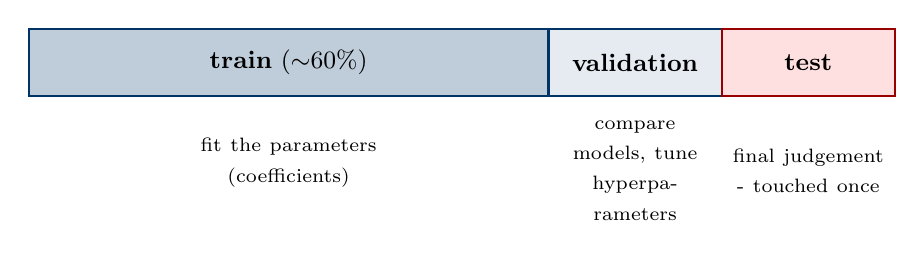
\begin{tikzpicture}[font=\small]
    \draw[fill=sghblue!25, draw=sghblue, thick] (0,0) rectangle (6.6,0.85);
    \draw[fill=sghblue!10, draw=sghblue, thick] (6.6,0) rectangle (8.8,0.85);
    \draw[fill=red!12, draw=red!60!black, thick] (8.8,0) rectangle (11,0.85);
    \node at (3.3,0.42) {\textbf{train} ($\sim$60\%)};
    \node at (7.7,0.42) {\textbf{validation}};
    \node at (9.9,0.42) {\textbf{test}};
    \node[align=center, text width=4.0cm] at (3.3,-0.85)
      {\scriptsize fit the parameters\\(coefficients)};
    \node[align=center, text width=2.0cm] at (7.7,-0.95)
      {\scriptsize compare models, tune hyperparameters};
    \node[align=center, text width=2.0cm] at (9.9,-0.95)
      {\scriptsize final judgement - \alert{touched once}};
  \end{tikzpicture}
  \end{center}
  \vspace{0.9em}
  \begin{itemize}\small
    \item Three questions, three datasets: \emph{what are the coefficients?}
          / \emph{which model or setting?} / \emph{how good is the winner,
          really?}
    \item Reusing one sample for two jobs is how optimism sneaks in -
          today's lab uses train + test only (no tuning yet); next week
          \alert{cross-validation} makes the validation job cheap.
  \end{itemize}
\end{frame}

% ============================================================
% SECTION: FROM INFERENCE TO PREDICTION
% ============================================================
\section{Prediction}

% ---------------------------------------------------------------
\begin{frame}{Same tool, new question}
  \begin{columns}[T]
    \begin{column}{0.5\textwidth}
      \textbf{Econometrics asks}
      \begin{itemize}\small
        \item is $\beta_1$ \emph{significant}? what is its causal story?
        \item standard errors, confidence intervals, tests
        \item the model explains the \emph{world}
      \end{itemize}
    \end{column}
    \begin{column}{0.5\textwidth}
      \textbf{Prediction asks}
      \begin{itemize}\small
        \item how accurate is $\hat{y}$ on \alert{customers we have never seen}?
        \item error on held-out data, stability over time
        \item the model supports a \emph{decision}
      \end{itemize}
    \end{column}
  \end{columns}
  \vspace{0.8em}
  \begin{center}
    Same $\hat\beta$'s, different loyalty. This course sits on the right -
    but borrows the left's discipline about interpretation.
  \end{center}
  \vspace{0.6em}
  \begin{center}\small
    On our portfolio: the econometrician asks \emph{``does a payment delay
    cause default?''}; we ask \emph{``is $\hat{P}(\text{default})$ accurate
    for tomorrow's applicants?''} - and both should ask \emph{``can I
    defend this model to a regulator?''}
  \end{center}
\end{frame}

% ---------------------------------------------------------------
\begin{frame}{Generalisation: the only score that counts}
  \begin{itemize}
    \item A model that perfectly reproduces its training data has proven one
          thing only: it can \alert{memorise}.
    \item The customer whose application arrives tomorrow is not in the
          training set. Performance on \emph{unseen} data - generalisation
          - is the product we sell.
    \item Everything in the next hour follows from one principle:
  \end{itemize}
  \vspace{0.6em}
  \begin{block}{The golden rule of prediction}
    Never judge a model on the data it was fitted on.
  \end{block}
  \vspace{0.4em}
  \begin{center}\small
    (Beginner trap \#1 from last week - now we build the defence.)
  \end{center}
\end{frame}

% ---------------------------------------------------------------
\begin{frame}{The train/test split}
  \textbf{The protocol}
  \begin{enumerate}\small
    \item Split once: e.g.\ 70\% \textbf{train}, 30\% \textbf{test}.
    \item Fit the model (and \emph{every} transform) on train only.
    \item Judge on test - and touch the test set \alert{as rarely as possible}.
  \end{enumerate}
  \vspace{0.5em}
  \textbf{Details that bite}
  \begin{itemize}\small
    \item \textbf{Stratify} classification splits: keep the default rate equal
          in both halves.
    \item \textbf{Fix the seed} (\texttt{random\_state}) - reproducibility,
          Block 1 style.
    \item Duplicates across the split = leakage (remember Block 1's keys check).
    \item With time-stamped data, split by \emph{time}, not at random -
          more in Block 3.
    \item 70/30 with no validation part? Fine \alert{today}: we tune nothing.
          The moment hyperparameters appear, carve validation out of the 70
          - or cross-validate (Block 3).
  \end{itemize}
\end{frame}

% ---------------------------------------------------------------
\begin{frame}[fragile]{The split, in code}
\small One import, one call - and two habits baked in:
{\footnotesize
\begin{semiverbatim}
from sklearn.model_selection import train_test_split

X_train, X_test, y_train, y_test = train_test_split(
    X, y,
    test_size=0.3,
    stratify=y,          \textit{\# same default rate in both halves}
    random_state=42,     \textit{\# reproducible split}
)
\end{semiverbatim}}
  \vspace{0.4em}
  \begin{itemize}\small
    \item From here on, \texttt{X\_test}, \texttt{y\_test} are locked in a
          drawer until judgement day.
    \item Every ``how good is it?'' during development must be answered
          \emph{without} them - that is what validation and (next week)
          cross-validation are for.
  \end{itemize}
\end{frame}

% ---------------------------------------------------------------
\begin{frame}{What overfitting looks like}
  \begin{center}
    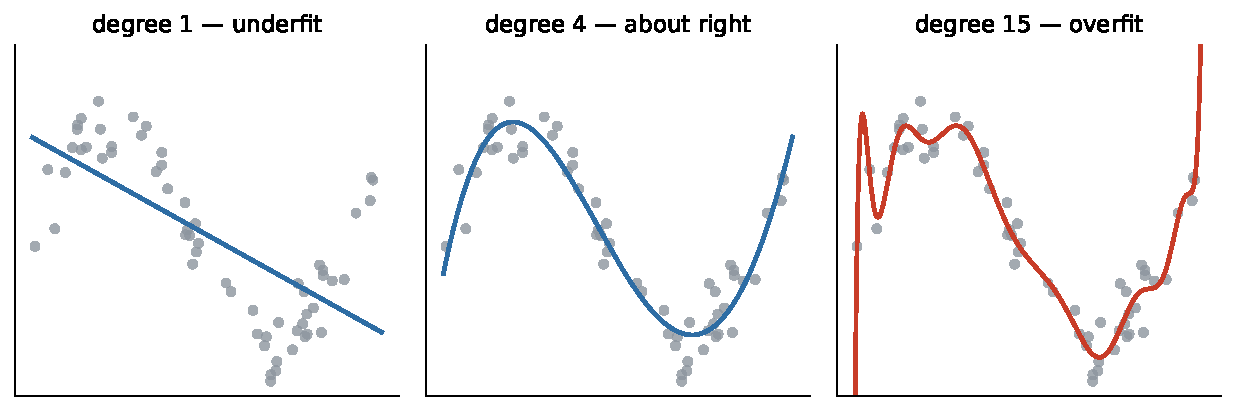
\includegraphics[width=0.94\textwidth]{figures/fig_overfitting.pdf}
  \end{center}
  \begin{itemize}\small
    \item Same data, three models. Degree 1 misses the structure
          (\alert{underfit}); degree 15 memorises the noise (\alert{overfit}).
    \item The overfit curve fits the training points \emph{best} - that is
          exactly why training error cannot be trusted.
  \end{itemize}
\end{frame}

% ---------------------------------------------------------------
\begin{frame}{The U-curve every model rides}
  \begin{center}
    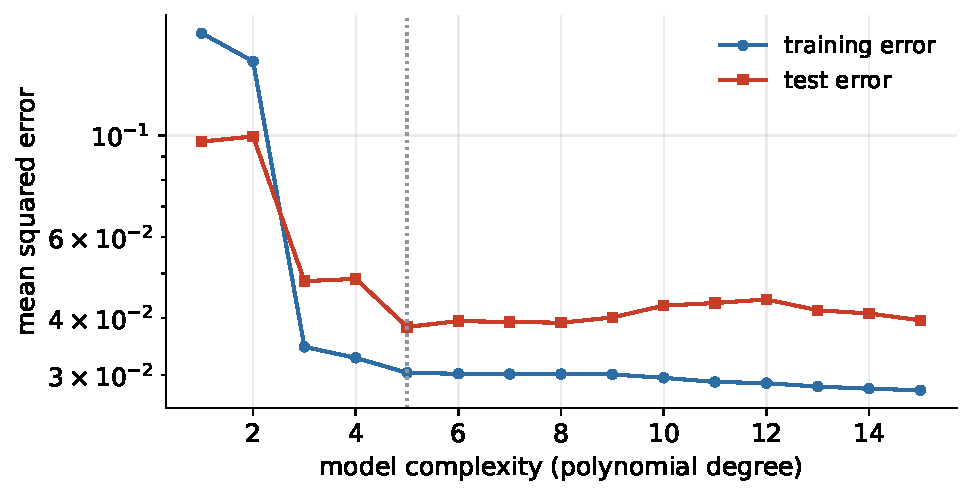
\includegraphics[width=0.66\textwidth]{figures/fig_bias_variance.pdf}
  \end{center}
  \begin{itemize}\small
    \item Training error only goes down with complexity; \alert{test error is
          a U} - underfitting on the left, overfitting on the right.
    \item Model selection = finding the bottom of the U \emph{without looking
          at the test set}. Regularisation (later today) is one steering wheel.
  \end{itemize}
\end{frame}

% ---------------------------------------------------------------
\begin{frame}{Two more ways to fool yourself}
  \textbf{Extrapolation}
  \begin{itemize}\small
    \item A model is trustworthy \emph{inside} the range of its training data.
    \item Our portfolio: credit limits up to 1M NT\$. A 5M NT\$ applicant?
          The model will output a number - \alert{confidently and baselessly}.
    \item (Selection bias from Block 1 makes this worse: approved customers
          only.)
  \end{itemize}
  \vspace{0.5em}
  \textbf{Test-set peeking}
  \begin{itemize}\small
    \item Check the test score, tweak the model, check again, tweak again\ldots
    \item Congratulations: you have manually fitted the test set. Its verdict
          is now \alert{contaminated}.
    \item Rule of thumb: the test set answers \emph{one} question, once,
          at the end.
  \end{itemize}
\end{frame}

% ============================================================
% SECTION: LINEAR REGRESSION
% ============================================================
\section{Linear regression}

% ---------------------------------------------------------------
\begin{frame}{The model}
  \[
    y \;=\; \beta_0 + \beta_1 x_1 + \beta_2 x_2 + \dots + \beta_k x_k + \varepsilon
  \]
  \begin{itemize}\small
    \item $y$ - numeric target (today's warm-up: \textbf{log payment});
          $x_j$ - features; $\varepsilon$ - what the features cannot explain.
    \item \textbf{Linear in the coefficients}, not in the world: $x_j$ can be
          $\log(\text{bill})$, an interaction flag, a squared term -
          feature engineering supplies the nonlinearity.
    \item Classical assumptions (independence, equal error variance,
          linearity) - we treat them as \alert{things to check with plots},
          not articles of faith. Residuals in three slides.
  \end{itemize}
\end{frame}

% ---------------------------------------------------------------
\begin{frame}{Least squares}
  Choose the coefficients that minimise the sum of squared mistakes:
  \[
    \min_{\beta}\; \sum_{i=1}^{n} \bigl(y_i - \hat{y}_i\bigr)^2,
    \qquad \hat{y}_i = \beta_0 + \beta_1 x_{i1} + \dots + \beta_k x_{ik}
  \]
  \begin{itemize}\small
    \item Why squares? Big misses hurt disproportionately, the objective is
          smooth, and the solution is a closed formula - no iteration needed.
    \item The price: squares make OLS \alert{sensitive to outliers} -
          one extreme customer can tilt the whole line (Block 1's boxplots
          just became modelling advice).
    \item Alternatives exist (absolute error, quantile regression) - good
          exam trivia, occasional real need.
  \end{itemize}
\end{frame}

% ---------------------------------------------------------------
\begin{frame}{Our first fit: payments vs bills}
  \begin{center}
    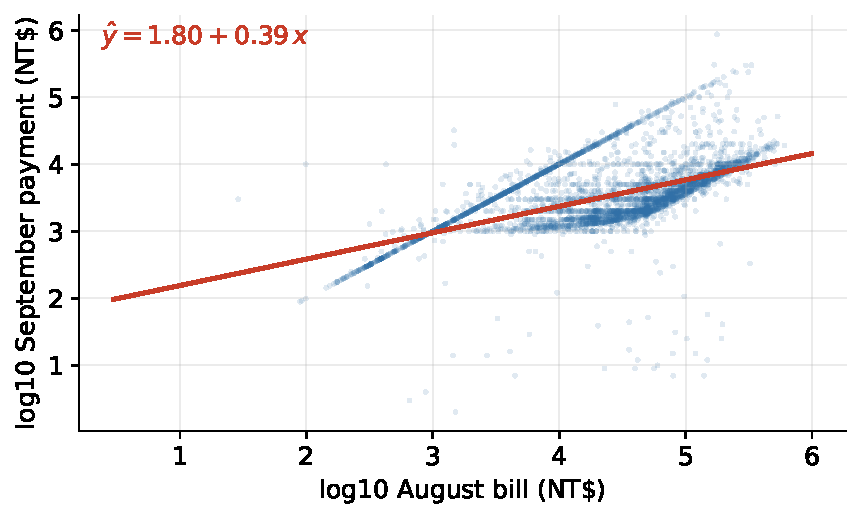
\includegraphics[width=0.56\textwidth]{figures/fig_linear_fit.pdf}
  \end{center}
  \begin{itemize}\small
    \item How much of last month's bill shows up in this month's payment?
          Log--log (Block 1's lens): the slope is an \alert{elasticity} -
          a 1\% larger bill draws only $\sim$\alert{0.39\%} more payment.
    \item Economics in one number: \alert{revolvers absorb the rest} -
          bigger bills are financed, not repaid. The cloud is wide; let's
          quantify how wide.
  \end{itemize}
\end{frame}

% ---------------------------------------------------------------
\begin{frame}{How good is the line? $R^2$, RMSE, MAE}
  \small
  \[
    R^2 = 1 - \frac{\sum_i (y_i-\hat{y}_i)^2}{\sum_i (y_i-\bar{y})^2}
    \qquad
    \mathrm{RMSE} = \sqrt{\tfrac{1}{n}\textstyle\sum_i (y_i-\hat{y}_i)^2}
    \qquad
    \mathrm{MAE} = \tfrac{1}{n}\textstyle\sum_i |y_i-\hat{y}_i|
  \]
  \vspace{0.2em}
  \begin{itemize}\small
    \item $R^2$: share of variance explained - unitless, comparable across
          targets. Our payment fit: $R^2 \approx 0.33$ on 24{,}605 paying
          customers.
    \item RMSE/MAE: in the \emph{units of the target} - the language for
          business (``we miss by X NT\$ on average''). RMSE punishes big
          misses; MAE is robust.
    \item \alert{Low $R^2$ is not failure}: real behavioural data is noisy,
          and a weak-but-real relationship can still price risk. The reverse
          matters more:
  \end{itemize}
  \vspace{0.3em}
  \begin{center}
    A \alert{suspiciously high} $R^2$ on behavioural data means leakage or a
    target twin - investigate before celebrating (Block 1, beginner traps).
  \end{center}
\end{frame}

% ---------------------------------------------------------------
\begin{frame}{Residuals tell the truth}
  \begin{center}
    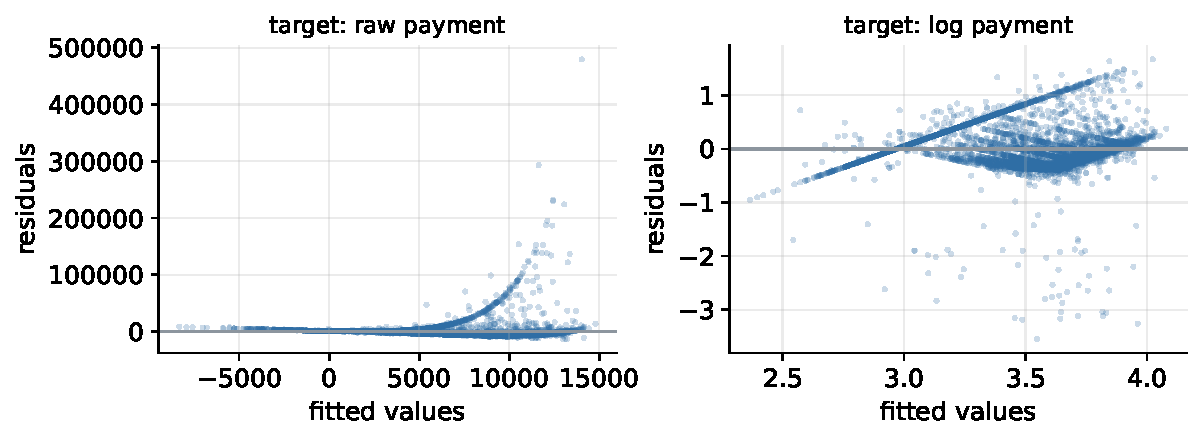
\includegraphics[width=0.92\textwidth]{figures/fig_residuals.pdf}
  \end{center}
  \begin{itemize}\small
    \item Residual $= y - \hat{y}$, plotted against the fitted value. You want
          a \alert{structureless band around zero}.
    \item Left (raw payments): a funnel - errors grow with the prediction
          (heteroscedasticity). Right (log payments): calm. \emph{The
          transform fixed the model, not just the histogram.}
    \item Curvature in this plot $\Rightarrow$ missing nonlinearity
          $\Rightarrow$ engineer a feature.
  \end{itemize}
\end{frame}

% ---------------------------------------------------------------
\begin{frame}{Reading coefficients without embarrassment}
  \begin{itemize}
    \item $\beta_j$ = expected change in $y$ per \alert{one unit} of $x_j$,
          \emph{holding the other features fixed} - units matter
          (per NT\$? per thousand? per SD?).
    \item To compare importance across features, \textbf{standardise} first
          (mean 0, SD 1): then $\beta_j$ = effect of one SD.
    \item Coefficients are \alert{teammates, not soloists}: adding or removing
          a correlated feature reshuffles the others (Block 1's correlation
          map warned you which ones).
    \item ``Holding fixed'' is a statistical statement, not a causal one -
          the Simpson's-paradox caution applies to coefficients too.
  \end{itemize}
\end{frame}

% ---------------------------------------------------------------
\begin{frame}{Categorical features enter the model: one-hot, carefully}
  \begin{itemize}\small
    \item One-hot from Block 1: \texttt{marriage} $\to$
          \texttt{marriage\_married}, \texttt{marriage\_single},
          \texttt{marriage\_other}.
    \item \textbf{Drop one level} (the \emph{reference}): with an intercept,
          all levels together are perfectly collinear - the
          \alert{dummy variable trap}.
    \item Each coefficient then reads ``\emph{versus the reference}'':
          $\beta_{\text{single}}$ = single vs married, all else fixed.
    \item Choose the reference deliberately (largest or most natural level) -
          it changes the story, not the fit.
  \end{itemize}
  \vspace{0.5em}
  \begin{center}\small
    Ordinal features (checking status): integer codes keep the order -
    but assert equal gaps. Your call, stated out loud.
  \end{center}
\end{frame}

% ---------------------------------------------------------------
\begin{frame}{Interactions: when one effect depends on another}
  \begin{center}
    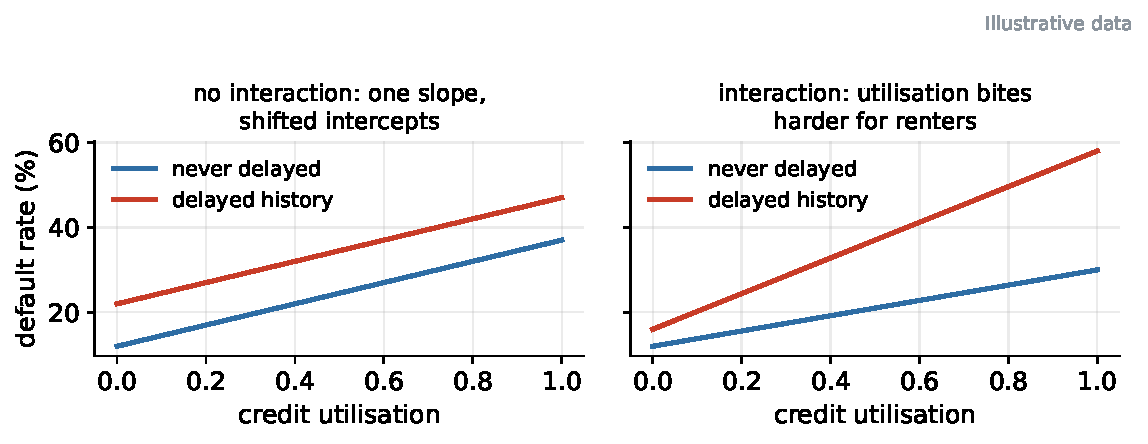
\includegraphics[width=0.76\textwidth]{figures/fig_interactions.pdf}
  \end{center}
  \vspace{-0.2em}
  \[
    y = \beta_0 + \beta_1\,\text{util} + \beta_2\,\text{delayed}
        + \alert{\beta_3\,(\text{util}\times\text{delayed})}
  \]
  \begin{itemize}\small
    \item With $\beta_3$: the slope of utilisation becomes
          $\beta_1 + \beta_3\,\text{delayed}$ - \alert{one feature moderates
          another}.
    \item A linear model cannot discover this on its own: the product column
          is \emph{feature engineering} (Block 1's interaction flag, graduated
          to a term). Trees find interactions automatically - next week.
  \end{itemize}
\end{frame}

% ---------------------------------------------------------------
\begin{frame}{Multicollinearity: correlated teammates}
  \begin{itemize}
    \item When two features carry near-identical information (recall
          $|r| > 0.8$ pairs from the Block 1 heatmap), OLS cannot decide how
          to split the credit between them.
    \item Symptoms: coefficients with \alert{absurd signs or sizes} that swing
          wildly between samples - while predictions stay fine.
    \item Consequence: \emph{prediction survives, interpretation dies}.
    \item Remedies: drop one twin, combine them (a ratio!), or
          \alert{regularise} - the third act of today.
  \end{itemize}
  \vspace{0.5em}
  \begin{center}\small
    Diagnostic keyword for the curious: variance inflation factor (VIF).
  \end{center}
\end{frame}

% ---------------------------------------------------------------
\begin{frame}{When the target is 0/1, the line breaks}
  \begin{center}
    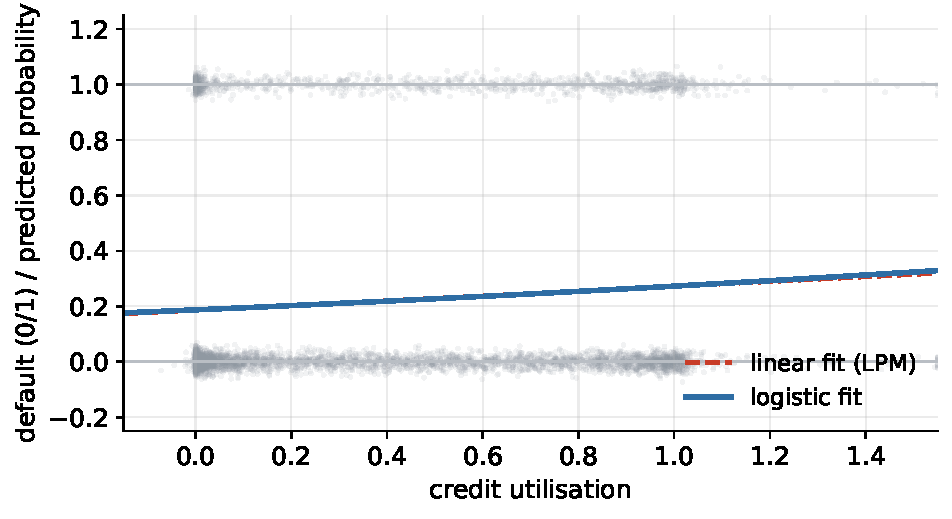
\includegraphics[width=0.67\textwidth]{figures/fig_lpm_vs_logistic.pdf}
  \end{center}
  \begin{itemize}\small
    \item Fit a straight line to \texttt{default}: predictions escape
          $[0,1]$ - ``$-$7\% probability'' and ``130\% probability''
          are not probabilities.
    \item We need a curve that \emph{lives} in $[0,1]$ and speaks probability
          natively. Enter the sigmoid.
  \end{itemize}
\end{frame}

% ============================================================
% SECTION: LOGISTIC REGRESSION
% ============================================================
\section{Logistic regression}

% ---------------------------------------------------------------
\begin{frame}{From line to S-curve}
  \begin{center}
    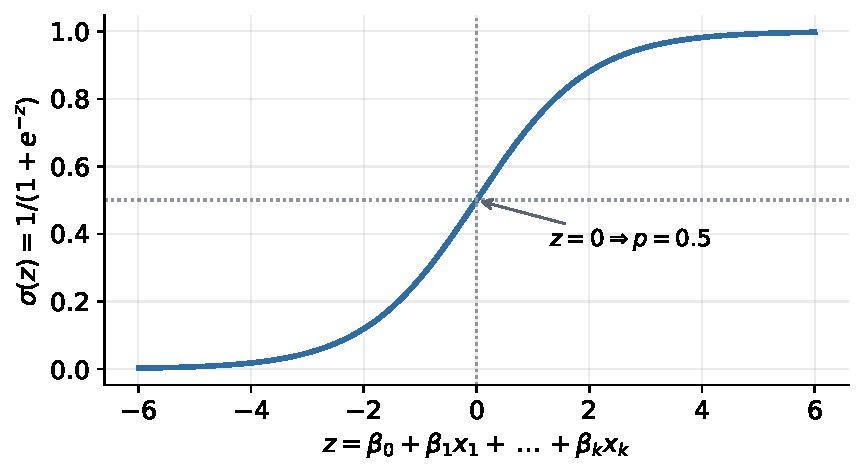
\includegraphics[width=0.62\textwidth]{figures/fig_sigmoid.pdf}
  \end{center}
  \begin{itemize}\small
    \item Keep the linear machinery $z = \beta_0 + \beta_1 x_1 + \dots$,
          then squash it: $p = \sigma(z) = 1/(1+e^{-z})$.
    \item Any score in $(-\infty, \infty)$ becomes a probability in $(0,1)$;
          the linear part still does all the thinking.
  \end{itemize}
\end{frame}

% ---------------------------------------------------------------
\begin{frame}{Odds and log-odds: the natural scale}
  \[
    \text{odds} = \frac{p}{1-p}
    \qquad\qquad
    \underbrace{\ln\frac{p}{1-p}}_{\text{log-odds (logit)}}
    = \beta_0 + \beta_1 x_1 + \dots + \beta_k x_k
  \]
  \vspace{0.2em}
  \begin{center}\small
  \begin{tabular}{@{}ccc@{}}
    \toprule
    probability $p$ & odds & log-odds \\
    \midrule
    0.10 & 1:9 $\;(0.11)$ & $-2.20$ \\
    0.50 & 1:1 $\;(1.00)$ & $0.00$ \\
    0.75 & 3:1 $\;(3.00)$ & $+1.10$ \\
    0.90 & 9:1 $\;(9.00)$ & $+2.20$ \\
    \bottomrule
  \end{tabular}
  \end{center}
  \vspace{0.3em}
  \begin{itemize}\small
    \item The model is \alert{linear in log-odds} - that is the sense in
          which logistic regression is a linear model.
    \item Bookmakers have spoken odds for centuries; credit scoring inherited
          the dialect.
  \end{itemize}
\end{frame}

% ---------------------------------------------------------------
\begin{frame}{Fitting: maximum likelihood, log-loss}
  No sum of squares this time - we choose $\beta$ to make the observed
  outcomes most probable:
  \[
    \min_{\beta}\;
    -\frac{1}{n}\sum_{i=1}^{n}\Bigl[\, y_i \ln \hat{p}_i
    + (1-y_i)\ln(1-\hat{p}_i) \Bigr]
    \qquad \text{(log-loss / cross-entropy)}
  \]
  \begin{itemize}\small
    \item Confidently wrong is punished brutally: predicting $\hat{p}=0.99$
          for a customer who repays costs $-\ln(0.01) \approx 4.6$; a humble
          $0.6$ costs $0.9$.
    \item No closed form - fitted iteratively. \texttt{sklearn} does this
          silently; you'll meet the same loss inside neural networks (Block 6).
    \item Same \texttt{fit}/\texttt{predict} API; plus
          \texttt{predict\_proba} for the probabilities themselves.
  \end{itemize}
\end{frame}

% ---------------------------------------------------------------
\begin{frame}{Our PD baseline: what the model learned}
  \begin{center}
    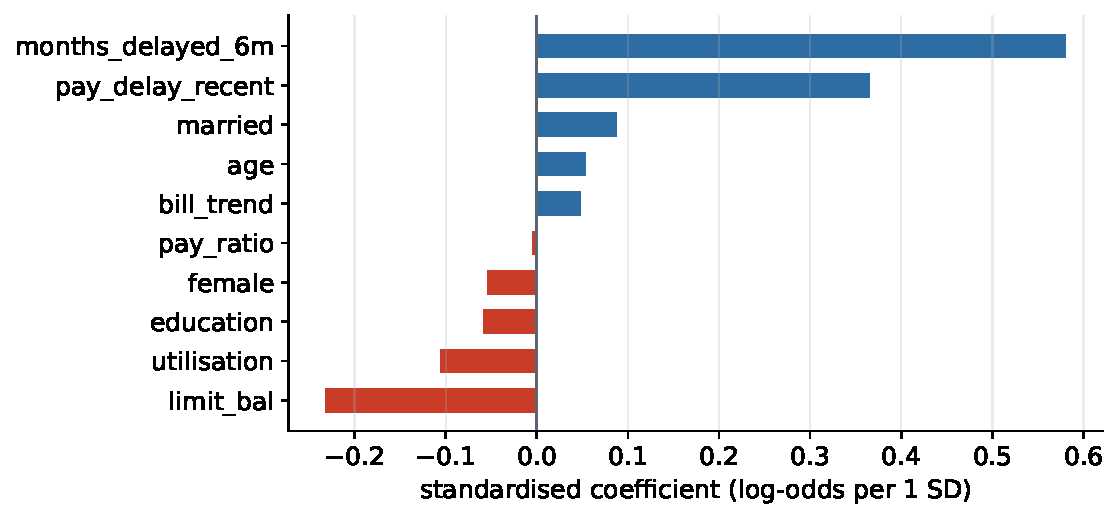
\includegraphics[width=0.68\textwidth]{figures/fig_logit_coefs.pdf}
  \end{center}
  \begin{itemize}\small
    \item \alert{Payment history is king}: the engineered delay counter
          \texttt{months\_delayed\_6m} ($+0.58$) and the most recent status
          ($+0.37$) tower over everything - Block 1's feature-engineering
          craft, vindicated on real data.
    \item And a haunting: \texttt{limit\_bal} at $-0.23$ - higher limits,
          \emph{lower} risk. The bank's \alert{old screening} granted big
          limits to safe clients: selection bias (Block 1), visible inside a
          coefficient.
  \end{itemize}
\end{frame}

% ---------------------------------------------------------------
\begin{frame}{Odds ratios: the language of credit}
  Exponentiate a coefficient and it becomes a \alert{multiplier of odds}:
  \[
    \text{odds}(x_j + \Delta) \;=\; e^{\beta_j \Delta} \cdot \text{odds}(x_j)
  \]
  \vspace{0.2em}
  \begin{itemize}\small
    \item Months delayed, $+1$ SD: odds of default
          $\times\, e^{0.58} \approx 1.8$.
    \item Credit limit, $+1$ SD: odds $\times\, e^{-0.23} \approx 0.79$ -
          a fifth of the odds gone (the screening echo, in odds language).
    \item Effects are \alert{multiplicative}: two $+1$ SD delay-moves
          compound to $1.8 \times 1.8 \approx 3.2$, not
          $+2\times$something.
  \end{itemize}
  \vspace{0.4em}
  \begin{center}\small
    ``The odds double per X points'' is exactly how scorecards talk -
    next slide.
  \end{center}
\end{frame}

% ---------------------------------------------------------------
\begin{frame}{Interpreting the model I: one customer, step by step}
  \begin{center}
    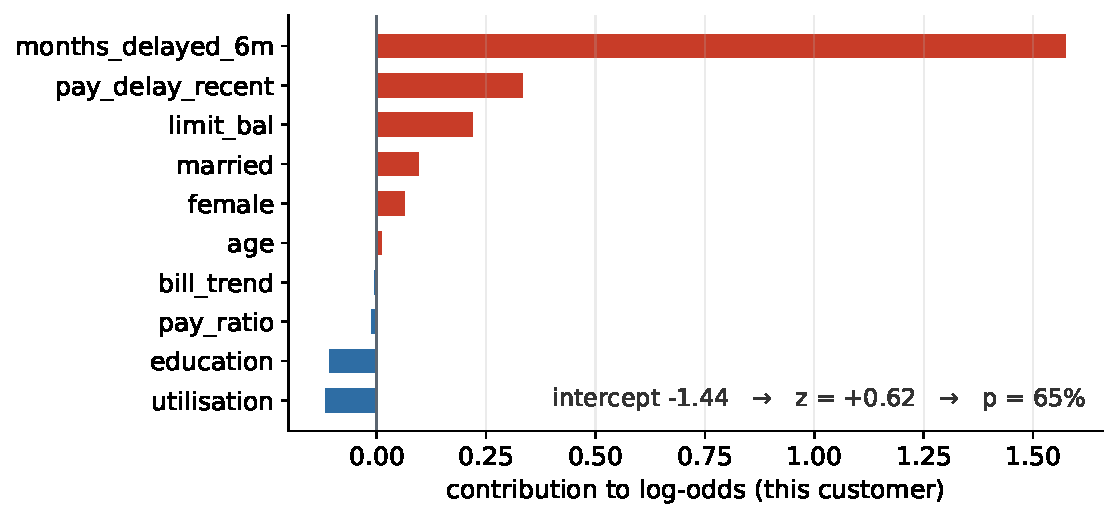
\includegraphics[width=0.65\textwidth]{figures/fig_customer_contrib.pdf}
  \end{center}
  \begin{itemize}\small
    \item Each bar $= \beta_j \times$ (this customer's standardised
          $x_j$): a full \alert{receipt} for one prediction -
          contributions sum, with the intercept, to $z$, and
          $\sigma(z)$ is the PD.
    \item Adverse-action reasons fall straight out: the largest red bars.
          For logistic regression this decomposition is \alert{exact and
          free} - SHAP (Block 3) exists to approximate it for models
          that aren't this polite.
  \end{itemize}
\end{frame}

% ---------------------------------------------------------------
\begin{frame}{Interpreting the model II: same odds ratio, different probability move}
  One SD more utilisation multiplies odds by $e^{0.43} \approx 1.54$ -
  \emph{for everyone}. On the probability scale, it does not move everyone
  equally:
  \vspace{0.3em}
  \begin{center}\small
  \begin{tabular}{@{}ccc@{}}
    \toprule
    PD before & PD after ($\text{odds} \times 1.54$) & change \\
    \midrule
    10\% & 14.6\% & $+4.6$ pp \\
    \alert{50\%} & \alert{60.6\%} & \alert{$+10.6$ pp} \\
    90\% & 93.3\% & $+3.3$ pp \\
    \bottomrule
  \end{tabular}
  \end{center}
  \vspace{0.4em}
  \begin{itemize}\small
    \item Near the tails the sigmoid is flat; near $p = 0.5$ it is steepest
          - marginal effect $\partial p / \partial x_j = \beta_j\,p(1-p)$.
    \item So: \alert{odds ratios are constant, probability effects are not}.
          Always say which scale you are on - and report probability
          changes in \emph{percentage points}, never ``percent''.
  \end{itemize}
\end{frame}

% ---------------------------------------------------------------
\begin{frame}{Scores, not probabilities: the scorecard tradition}
  \begin{itemize}
    \item A credit score is a \alert{rescaled log-odds}: pick a base score,
          pick ``points to double the odds'' (say 20), done.
          Linear in the same $z$ our model computes.
    \item Why banks kept it: additive per-feature points (from WoE-encoded
          bins, Block 1's encodings slide) are auditable line by line -
          each feature's contribution is a number a regulator can read.
    \item Logistic regression + WoE + scorecard formatting \emph{is} the
          classical credit-scoring stack - decades old, still in production
          everywhere.
  \end{itemize}
  \vspace{0.5em}
  \begin{center}\small
    Modern practice: GBDT for power (next week), logistic scorecard for
    explainability - often both, side by side.
  \end{center}
\end{frame}

% ---------------------------------------------------------------
\begin{frame}{From probability to decision}
  \begin{center}
    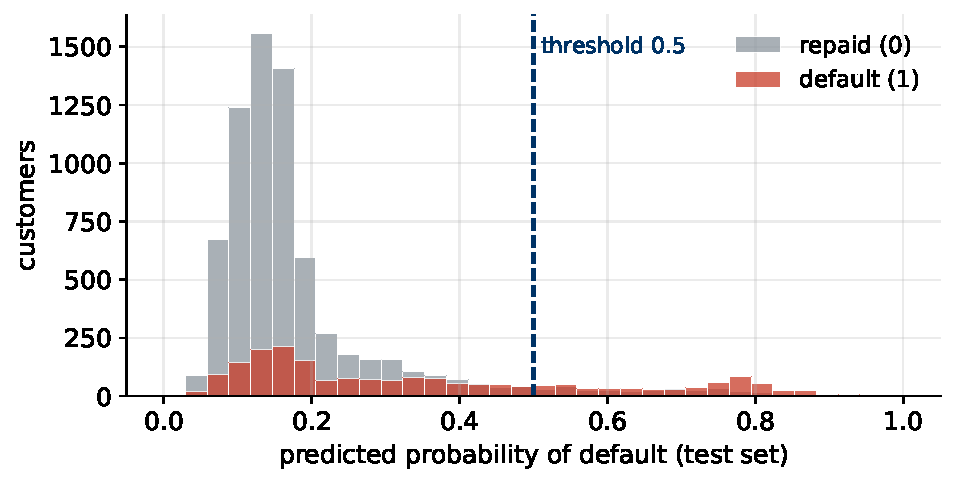
\includegraphics[width=0.67\textwidth]{figures/fig_pred_prob_hist.pdf}
  \end{center}
  \begin{itemize}\small
    \item The two classes \alert{overlap} - no threshold separates them
          cleanly; every cut-off trades one error for another.
    \item $0.5$ is not a law of nature; it is \texttt{sklearn}'s default.
          The right threshold comes from \emph{costs} - end of this block.
  \end{itemize}
\end{frame}

% ---------------------------------------------------------------
\begin{frame}{Class imbalance: three honest notes}
  \begin{enumerate}
    \item Our 22\% default rate is friendly; loan-book PD data (1--5\%) pushes
          predicted probabilities low - at threshold 0.5 such a model may
          \alert{never} predict ``default''. That is a threshold problem,
          not a model problem.
    \item \texttt{class\_weight="balanced"} re-weights the loss - useful,
          but it \alert{distorts predicted probabilities}; recalibration
          needed if probabilities matter (they do, in pricing).
    \item Resampling (over/under-sampling) is popular and overrated -
          try thresholds and weights first.
  \end{enumerate}
  \vspace{0.4em}
  \begin{center}\small
    Calibration - ``is a predicted 0.3 really a 0.3?'' - gets proper
    treatment in Block 3.
  \end{center}
\end{frame}

% ---------------------------------------------------------------
\begin{frame}{Why logistic regression is \emph{the} baseline}
  \begin{itemize}
    \item \textbf{Fast}: fits in milliseconds, scales to millions of rows.
    \item \textbf{Stable}: no tuning required to be decent.
    \item \textbf{Explainable}: coefficients $\to$ odds ratios $\to$
          adverse-action reasons; regulators approve.
    \item \textbf{Honest yardstick}: any complex model must \alert{earn its
          complexity} by beating this - measurably, on held-out data.
  \end{itemize}
  \vspace{0.6em}
  \begin{block}{The baseline discipline}
    No GBDT, no neural network, no ensemble gets built in this course -
    or in your projects - before a logistic baseline exists.
  \end{block}
\end{frame}

% ---------------------------------------------------------------
\begin{frame}{Linear vs logistic, side by side}
  \small
  \begin{center}
  \begin{tabular}{@{}lll@{}}
    \toprule
     & Linear regression & Logistic regression \\
    \midrule
    Target & numeric & binary (0/1) \\
    Output & a number, unbounded & probability in $(0,1)$ \\
    Linear in & the target & the \emph{log-odds} \\
    Fitted by & least squares (closed form) & max.\ likelihood (iterative) \\
    Loss & squared error & log-loss \\
    Read effects as & units of $y$ per unit $x$ & odds ratio $e^{\beta}$ \\
    Credit use & LGD, exposure, income est. & \alert{PD - the core task} \\
    \bottomrule
  \end{tabular}
  \end{center}
  \vspace{0.5em}
  \begin{center}
    One family, two dialects. Master both, and Block 3's models are
    ``just'' better function shapes.
  \end{center}
\end{frame}

% ============================================================
% SECTION: REGULARISATION
% ============================================================
\section{Regularisation}

% ---------------------------------------------------------------
\begin{frame}{Why shrink coefficients on purpose?}
  \begin{itemize}
    \item Many features + correlated features + finite data $\Rightarrow$
          coefficients tailored to \alert{this sample's noise} -
          the overfitting U-curve, wearing a suit.
    \item Idea: add a \alert{penalty for large coefficients} to the loss.
          The model must now buy each unit of coefficient with genuine
          predictive payoff.
    \item Price and prize: a little bias in, a lot of variance out -
          usually a bargain on test error.
  \end{itemize}
  \vspace{0.5em}
  \begin{center}
    Two classic penalties, two personalities: ridge and lasso.
  \end{center}
\end{frame}

% ---------------------------------------------------------------
\begin{frame}{Ridge (L2): smooth shrinkage}
  \begin{columns}[T]
    \begin{column}{0.38\textwidth}
      \vspace{1.2em}
      {\small
      \[
        \min_{\beta}\; \sum_{i}(y_i-\hat{y}_i)^2 + \alpha \sum_{j} \beta_j^2
      \]}
      \begin{itemize}\small
        \item As $\alpha$ grows, every coefficient shrinks toward zero -
              smoothly, \alert{never exactly to zero}.
        \item Loves correlated features: splits credit between twins instead
              of gambling on one. The multicollinearity remedy.
      \end{itemize}
    \end{column}
    \begin{column}{0.6\textwidth}
      \begin{center}
        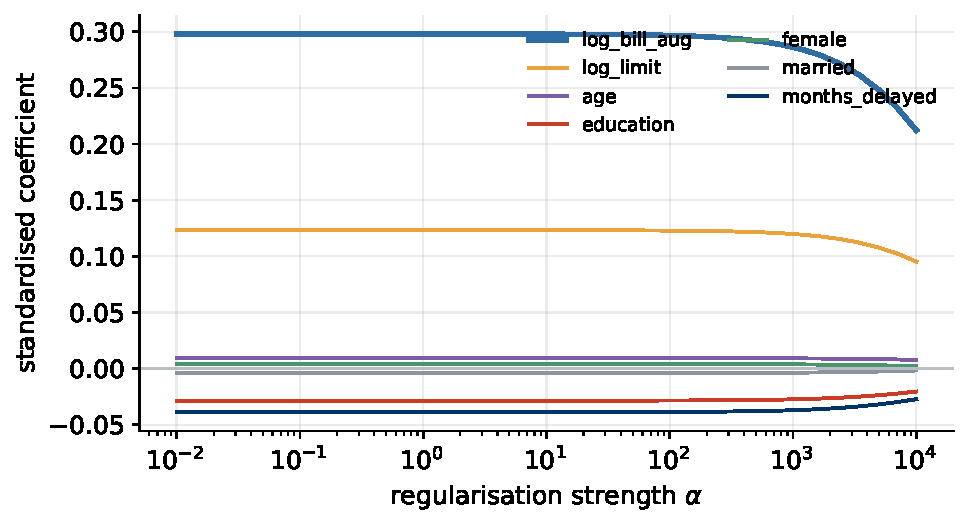
\includegraphics[width=\linewidth]{figures/fig_ridge_paths.pdf}
      \end{center}
    \end{column}
  \end{columns}
\end{frame}

% ---------------------------------------------------------------
\begin{frame}{Lasso (L1): shrinkage with a guillotine}
  \begin{columns}[T]
    \begin{column}{0.38\textwidth}
      \vspace{1.2em}
      {\small
      \[
        \min_{\beta}\; \sum_{i}(y_i-\hat{y}_i)^2 + \alpha \sum_{j} |\beta_j|
      \]}
      \begin{itemize}\small
        \item Coefficients hit \alert{exactly zero} one by one - built-in
              feature selection; the survivors are your shortlist.
        \item With twin features it tends to keep one and drop the other -
              convenient, but don't read the choice causally.
        \item Mind the $\alpha$ axis: L1 bites at much smaller $\alpha$
              than ridge did.
      \end{itemize}
    \end{column}
    \begin{column}{0.6\textwidth}
      \begin{center}
        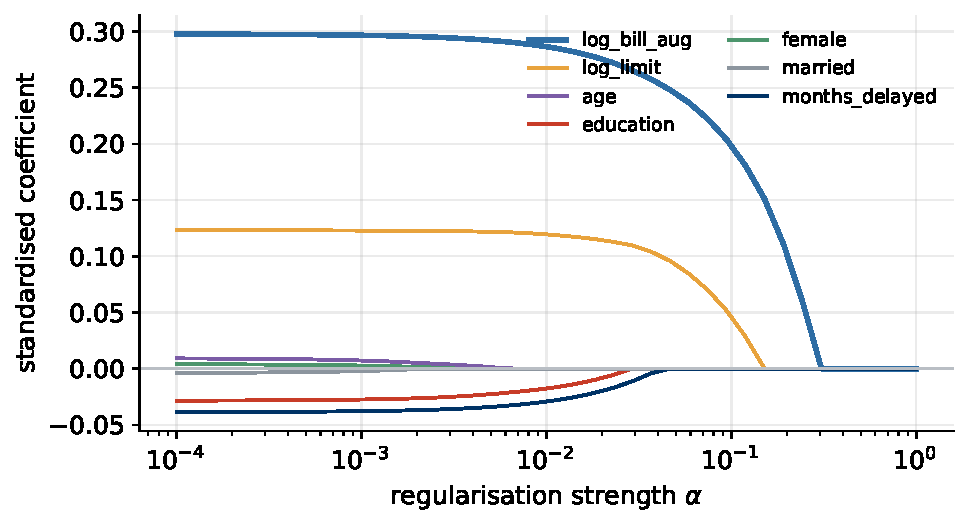
\includegraphics[width=\linewidth]{figures/fig_lasso_paths.pdf}
      \end{center}
    \end{column}
  \end{columns}
\end{frame}

% ---------------------------------------------------------------
\begin{frame}{Why the guillotine: the geometry of L1 vs L2}
  \begin{center}
    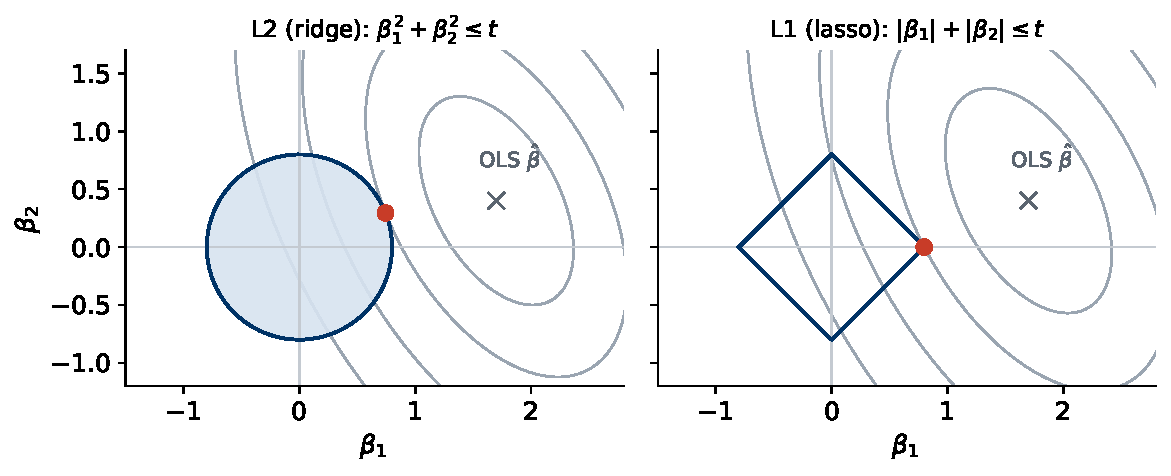
\includegraphics[width=0.8\textwidth]{figures/fig_l1_l2_geometry.pdf}
  \end{center}
  \begin{itemize}\small
    \item Grey ellipses: equal-loss curves around the unpenalised OLS
          solution. Shaded region: the \alert{coefficient budget} the penalty
          allows. The solution is the first touch.
    \item A circle can be touched anywhere $\Rightarrow$ ridge coefficients
          get \emph{small}, not zero. A diamond gets hit at its
          \alert{corners} - and corners have $\beta_j = 0$ exactly.
  \end{itemize}
\end{frame}

% ---------------------------------------------------------------
\begin{frame}{Scale first, or the penalty is nonsense}
  \begin{itemize}
    \item The penalty charges by \alert{coefficient size} - and size depends
          on units. Limit-in-NT\$ gets a tiny coefficient, age-in-years a
          big one, for identical importance.
    \item Unscaled features $\Rightarrow$ the penalty punishes features for
          their \emph{units}, not their usefulness.
    \item Standard fix: \texttt{StandardScaler} (mean 0, SD 1) before any
          penalised model.
    \item And the Block 1 golden rule again: the scaler's mean and SD are
          \alert{fitted on train only} - test data must not leak into them.
  \end{itemize}
  \vspace{0.5em}
  \begin{center}\small
    ``But sklearn didn't warn me'' - correct, it won't. This one is on you.
  \end{center}
\end{frame}

% ---------------------------------------------------------------
\begin{frame}{Choosing $\alpha$: validation, not vibes}
  \begin{center}
    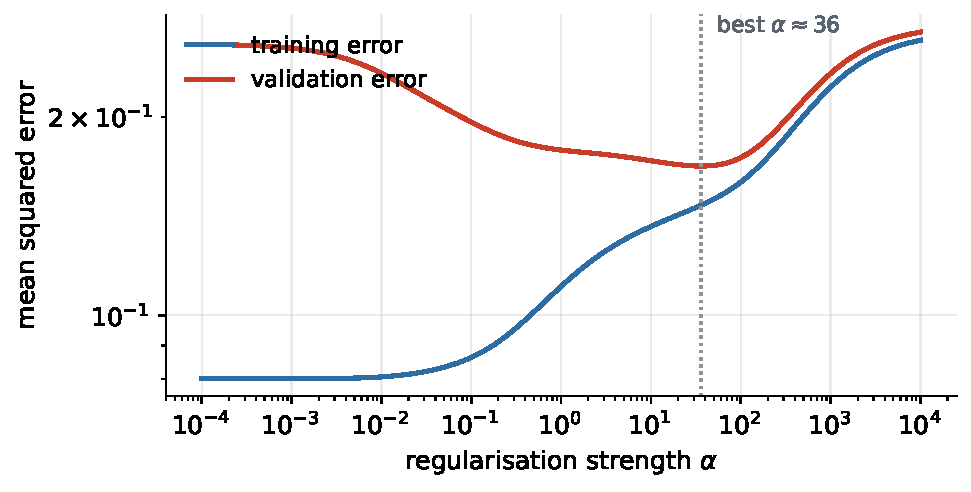
\includegraphics[width=0.68\textwidth]{figures/fig_validation_curve.pdf}
  \end{center}
  \begin{itemize}\small
    \item $\alpha$ is a \alert{hyperparameter}: the data used to fit
          coefficients cannot also pick it.
    \item Sweep $\alpha$, judge on held-out data, take the bottom of the U.
          Done properly (cross-validation) next week.
  \end{itemize}
\end{frame}

% ---------------------------------------------------------------
\begin{frame}{Regularisation: practical notes}
  \begin{itemize}
    \item \textbf{Elastic net} = ridge + lasso mixed; when in doubt between
          them, mix.
    \item \textbf{Gotcha}: in \texttt{LogisticRegression} the knob is
          \texttt{C} $= 1/\alpha$ - \alert{bigger C = weaker penalty} -
          and regularisation is \alert{on by default} (\texttt{C=1}).
          You have been regularising all along without knowing.
    \item Ridge/lasso logic transfers to logistic regression unchanged
          (penalise the same $\beta$'s under log-loss).
    \item Regularisation controls \emph{coefficients}, not data quality:
          it will happily shrink its way around leakage without curing it.
  \end{itemize}
\end{frame}

% ---------------------------------------------------------------
\begin{frame}{Regularisation is everywhere (a preview)}
  Penalties are one instance of a universal idea: \alert{put a leash on
  flexibility, and generalisation improves}.
  \vspace{0.3em}
  \small
  \begin{center}
  \begin{tabular}{@{}lll@{}}
    \toprule
    Leash & Model family & Where in this course \\
    \midrule
    L1 / L2 penalty & linear \& logistic & today \\
    Max depth, min leaf size & decision trees & Block 3 \\
    Fewer boosting rounds, learning rate & GBDT & Block 3 \\
    Early stopping, dropout & neural networks & Block 6 \\
    Coarse bins (WoE) & scorecards & Blocks 1--2 \\
    \bottomrule
  \end{tabular}
  \end{center}
  \vspace{0.5em}
  \begin{itemize}\small
    \item Different mechanics, one U-curve: each knob trades training fit
          for test stability.
    \item When you meet a new model family, your first question is now
          fixed: \alert{``where is its leash?''}
  \end{itemize}
\end{frame}

% ---------------------------------------------------------------
\begin{frame}[fragile]{The leakage-safe pattern: Pipeline}
\small Weld the preprocessing to the model:
{\footnotesize
\begin{semiverbatim}
from sklearn.pipeline import make_pipeline
from sklearn.preprocessing import StandardScaler
from sklearn.linear_model import LogisticRegression

pipe = make_pipeline(StandardScaler(),
                     LogisticRegression(max_iter=2000))
pipe.fit(X_train, y_train)           \textit{\# scaler fitted on train ONLY}
proba = pipe.predict_proba(X_test)[:, 1]
\end{semiverbatim}}
  \vspace{0.4em}
  \begin{itemize}\small
    \item The pipeline welds preprocessing to the model: whatever data the
          model sees, the transforms were fitted on \emph{its training part}.
    \item This is not style advice - next week, inside cross-validation,
          pipelines are the \alert{only} way to stay leakage-free.
  \end{itemize}
\end{frame}

% ============================================================
% SECTION: EVALUATION, PART 1
% ============================================================
\section{Evaluation I}

% ---------------------------------------------------------------
\begin{frame}{The accuracy trap, now with our own numbers}
  Our PD baseline on the held-out test set (9{,}000 real clients):
  \begin{center}
  \begin{tabular}{@{}lc@{}}
    \toprule
    Model & Accuracy \\
    \midrule
    Always predict ``repaid'' & 77.9\% \\
    Our logistic baseline (threshold 0.5) & \alert{80.6\%} \\
    \bottomrule
  \end{tabular}
  \end{center}
  \vspace{0.5em}
  \begin{itemize}\small
    \item Three points better than a model that \emph{does nothing}.
          Is our model useless?
    \item No - it \alert{ranks} customers well; accuracy at an arbitrary
          threshold just cannot see it.
    \item Diagnosis requires opening the black box of ``right and wrong''
          - next slide.
  \end{itemize}
\end{frame}

% ---------------------------------------------------------------
\begin{frame}{The confusion matrix}
  \begin{center}
  \small
  \begin{tabular}{@{}ll|cc@{}}
    \toprule
    & & \multicolumn{2}{c}{\textbf{Predicted}} \\
    & & default & repaid \\
    \midrule
    \multirow{2}{*}{\textbf{Actual}}
    & default & \textbf{TP = 541} \; caught & \alert{\textbf{FN = 1{,}450}} \; missed \\
    & repaid  & \alert{\textbf{FP = 294}} \; falsely declined & \textbf{TN = 6{,}715} \; rightly approved \\
    \bottomrule
  \end{tabular}
  \end{center}
  \vspace{0.5em}
  \begin{itemize}\small
    \item Four numbers, four different business events - \alert{never} let
          them collapse into one ``accuracy'' without looking.
    \item Our baseline at 0.5: cautious - it declines rarely (294 false
          alarms) but \alert{misses 1{,}450 of 1{,}991 defaulters}.
  \end{itemize}
\end{frame}

% ---------------------------------------------------------------
\begin{frame}{Errors have price tags - different ones}
  \begin{columns}[T]
    \begin{column}{0.5\textwidth}
      \textbf{False negative} (missed defaulter)
      \begin{itemize}\small
        \item loan granted, money lost
        \item cost $\sim$ the \alert{principal}
      \end{itemize}
    \end{column}
    \begin{column}{0.5\textwidth}
      \textbf{False positive} (good customer declined)
      \begin{itemize}\small
        \item margin lost, customer possibly gone for good
        \item cost $\sim$ the \emph{margin}
      \end{itemize}
    \end{column}
  \end{columns}
  \vspace{0.7em}
  \begin{itemize}\small
    \item The two costs differ by an \alert{order of magnitude} - and the
          ratio belongs to the business, not to the data scientist.
    \item A model tuned for symmetric errors is tuned for a fictional bank.
    \item This asymmetry, not mathematics, will pick our threshold.
  \end{itemize}
\end{frame}

% ---------------------------------------------------------------
\begin{frame}{Precision and recall}
  \[
    \text{precision} = \frac{TP}{TP + FP}
    \qquad\qquad
    \text{recall} = \frac{TP}{TP + FN}
  \]
  \vspace{0.2em}
  \begin{itemize}\small
    \item \textbf{Precision}: when we flag a defaulter, how often are we
          right? Ours: $541/835 \approx \alert{65\%}$ - against a 22\%
          base rate, that is real skill.
    \item \textbf{Recall}: of all true defaulters, how many do we catch?
          Ours: $541/1991 \approx \alert{27\%}$ - nearly three out of four
          walk through.
    \item The pair always trades off - and the exchange rate is the
          threshold.
  \end{itemize}
  \vspace{0.4em}
  \begin{center}\small
    (F1 = harmonic mean of the two - one number, both flavours, and blind to
    costs and true negatives. Use knowingly or not at all.)
  \end{center}
\end{frame}

% ---------------------------------------------------------------
\begin{frame}{Move the threshold, move the business}
  \begin{center}
    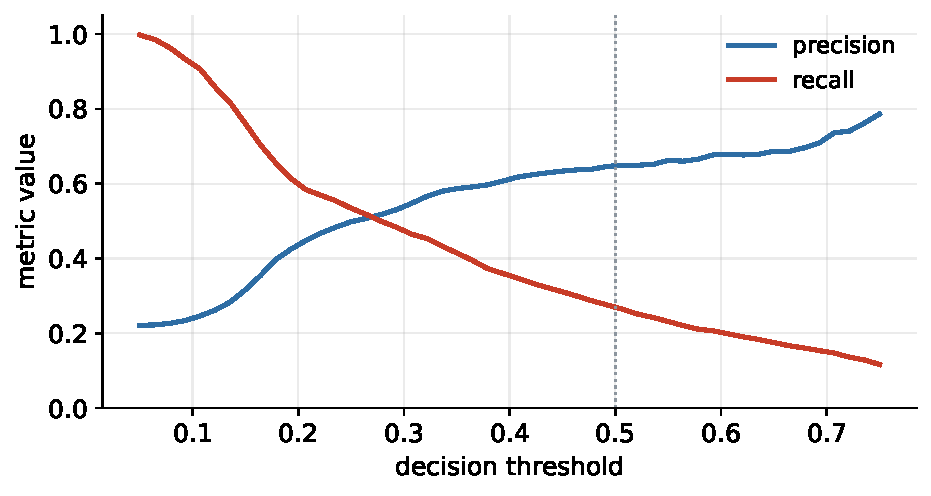
\includegraphics[width=0.7\textwidth]{figures/fig_threshold_tradeoff.pdf}
  \end{center}
  \begin{itemize}\small
    \item Lower the threshold: catch more defaulters (recall $\uparrow$),
          decline more good customers (precision $\downarrow$).
    \item The threshold is a \alert{business decision} expressed in code -
          risk appetite, not arithmetic.
  \end{itemize}
\end{frame}

% ---------------------------------------------------------------
\begin{frame}{Which metric for PD, then?}
  \begin{itemize}
    \item \textbf{Accuracy}: no. (You have seen why, twice.)
    \item \textbf{Precision/recall}: honest but \alert{threshold-bound} -
          they judge one cut-off, not the model.
    \item What we actually want to know, in order:
    \begin{enumerate}\small
      \item Does the model \emph{rank} risk well? $\to$ ROC / AUC
            (next week)
      \item Are the probabilities \emph{honest}? $\to$ calibration
            (next week)
      \item What does the best threshold \emph{earn}? $\to$ expected-cost
            analysis (next week, with your numbers)
    \end{enumerate}
    \item Until then, one rule survives every situation:
          \alert{never a single metric, never on training data}.
  \end{itemize}
\end{frame}

% ============================================================
% SECTION: LAB
% ============================================================
\section{Lab}

% ---------------------------------------------------------------
\begin{frame}[plain]
  \begin{center}
    \vspace{1.5cm}
    {\LARGE\textbf{Laboratory}}\\[0.6cm]
    {\normalsize Notebook \texttt{02\_regression\_baselines} - laptops out.}
  \end{center}
\end{frame}

% ---------------------------------------------------------------
\begin{frame}{Lab today}
  \begin{columns}[T]
    \begin{column}{0.52\textwidth}
      \textbf{Notebook \texttt{02\_regression\_baselines}}
      \begin{itemize}\small
        \item split the portfolio (stratified, seeded)
        \item linear warm-up: payments from bills
        \item logistic PD baseline in a pipeline
        \item read coefficients \& odds ratios
        \item play the threshold game
      \end{itemize}
    \end{column}
    \begin{column}{0.48\textwidth}
      \textbf{Done =}
      \begin{itemize}\small
        \item you can defend your baseline: features used, one number you
              trust, and \emph{why} that number
        \item you know your model's confusion matrix at two thresholds
      \end{itemize}
    \end{column}
  \end{columns}
\end{frame}

% ============================================================
% SECTION: SUMMARY
% ============================================================
\section{Summary}

% ---------------------------------------------------------------
\begin{frame}[plain]
  \begin{center}
    \vspace{1.5cm}
    {\LARGE\textbf{Summary}}\\[0.6cm]
    {\normalsize What to take home from Block 2.}
  \end{center}
\end{frame}

% ---------------------------------------------------------------
\begin{frame}{Block 2 in five sentences}
  \begin{enumerate}
    \item Judge models only on \textbf{unseen data} - the train/test split
          is the minimum honest protocol.
    \item Linear regression predicts numbers; its coefficients are
          \textbf{unit-bound teammates}, and residual plots tell the truth.
    \item Logistic regression is linear in \textbf{log-odds}; $e^{\beta}$
          multiplies odds, which is exactly how credit talks.
    \item \textbf{Regularisation} (ridge smoothly, lasso to zero) buys test
          error with bias - after scaling, chosen by validation.
    \item Accuracy lies under imbalance; read the \textbf{confusion matrix},
          price its cells, and treat the \textbf{threshold} as a business
          decision.
  \end{enumerate}
\end{frame}

% ---------------------------------------------------------------
\begin{frame}{Project status \& reminder}
  \begin{itemize}
    \item Teams of 3 closed \alert{today at 17:10} - not in one? Talk to me
          in the break, we fix it now.
    \item \alert{Before Block 3 (20.10): topic + short written description}
          - the decision, the dataset, the target, the planned two model
          families. No idea? \textbf{Consult before the deadline}.
    \item One of your two families should probably be today's logistic
          baseline - cheap, defensible, expected.
  \end{itemize}
  \vspace{0.6em}
  \begin{center}\small
    Rubric reminder: ``Modelling: $\geq$2 families, justified'' is 15\% -
    and ``justified'' means \emph{against a baseline}.
  \end{center}
\end{frame}

% ---------------------------------------------------------------
\begin{frame}{Exam practice - multiple choice}
  \small
  \textbf{Q1.} A standardised logistic coefficient for
  \texttt{months\_delayed\_6m} is $+0.6$. The correct reading:
  \begin{enumerate}[(a)]
    \item default probability rises by 0.6 pp per month of delay
    \item one SD more delay adds $0.6$ to the log-odds - odds $\times\,e^{0.6}\approx 1.8$
    \item default probability multiplies by 1.8 for every customer
    \item the feature explains 60\% of defaults
  \end{enumerate}
  \vspace{0.4em}
  \textbf{Q2.} Why must the scaler live \emph{inside} the pipeline, fitted on
  training data only?
  \begin{enumerate}[(a)]
    \item it makes the code shorter
    \item fitting it on all rows lets test-set statistics leak into training
    \item scaling the test set is forbidden
    \item scikit-learn refuses to fit it otherwise
  \end{enumerate}
\end{frame}
% Answer key: Q1 (b) - constant on the odds scale, NOT on the probability
% scale (the sigmoid bends). Q2 (b) - the golden rule applies to
% preprocessing too; the test set must contribute nothing to fitting.

% ---------------------------------------------------------------
\begin{frame}{Exam practice - open question}
  \begin{block}{In the style of the term-0 exam ($\sim$60\% open questions)}
    At threshold 0.5 your PD baseline catches 27\% of defaulters at 65\%
    precision; at threshold 0.30 it catches far more defaulters at visibly
    lower precision. A manager asks: ``which threshold is correct?''
    Answer in 4-6 sentences.
  \end{block}
  \vspace{0.5em}
  \begin{center}\small
    Hint: the best answers contain no model mathematics at all.
  \end{center}
\end{frame}
% A good answer: neither is "correct" - the threshold trades missed
% defaulters (FN) against declined good customers (FP), and the right
% exchange rate is the business's cost ratio, not a statistical constant.
% 0.5 is a software default, not a law. State the costs, then the threshold
% follows (Block 3 prices this exactly with the expected-cost curve).

% ---------------------------------------------------------------
\begin{frame}[plain]
  \begin{center}
    \vspace{1.5cm}
    {\LARGE\textbf{Next week: trees, ensembles \& honest evaluation.}}\\[0.6cm]
    {\normalsize The \texttt{collections\_contact} trap finally springs -
    live.}
  \end{center}
\end{frame}

% ---------------------------------------------------------------
\begin{frame}{Keep learning - Block 2 reading}
  \begin{itemize}
    \item \textbf{Shmueli} - \emph{To Explain or to Predict?}
          (Statistical Science, 2010) - the inference-vs-prediction
          re-framing, in one readable paper.
    \item \textbf{Tibshirani} - \emph{Regression Shrinkage and Selection
          via the Lasso} (JRSS-B, 1996) - the original lasso paper; the
          geometry slide, from the source.
    \item \textbf{Hand \& Henley} - \emph{Statistical Classification
          Methods in Consumer Credit Scoring: a Review} (JRSS-A, 1997) -
          the scorecard tradition our odds-ratio talk descends from.
    \item \textbf{scikit-learn User Guide} - \emph{Linear models} section:
          regularisation explained better than most textbooks.
  \end{itemize}
\end{frame}

\end{document}
